\documentclass[10pt,twocolumn,letterpaper]{article}
\usepackage{cvpr}  % camera-ready layout of the official CVPR author kit

\usepackage{graphicx}
\usepackage{amsmath}
\usepackage{amssymb}
\usepackage{booktabs}
\usepackage{multirow}
\usepackage{xcolor}
\definecolor{cvprblue}{rgb}{0.21,0.49,0.74}
\usepackage[pagebackref,breaklinks,colorlinks,allcolors=cvprblue]{hyperref}

\def\paperID{ML-Project}
\def\confName{CVPR}
\def\confYear{2026}

% ---- links filled in after publishing (see README) ----
\newcommand{\repoURL}{\url{https://github.com/GITHUB_USER/GITHUB_REPO}}
\newcommand{\hfURL}{\url{https://huggingface.co/HF_REPO_ID}}

\newcommand{\best}[1]{\textbf{#1}}
\newcommand{\pmstd}[1]{{\scriptsize$\pm$#1}}

\title{YOLO-Backbone-Guided Conditional Diffusion for Polyp Segmentation:\\
Does Iterative Denoising Help Cross-Dataset Generalization?}

\author{Prashant Kumar Mittra\\
IIT Jodhpur\\
{\tt\small m24ma2009@iitj.ac.in}
\and
Pawan Kumar Koli\\
IIT Jodhpur\\
{\tt\small m24ma2007@iitj.ac.in}
\and
Deep Das\\
IIT Jodhpur\\
{\tt\small m26mac004@iitj.ac.in}
}

\begin{document}
\maketitle

% =====================================================================
\begin{abstract}
Polyp segmentation models trained on one colonoscopy dataset lose accuracy on images from another. We study this cross-dataset gap with a conditional diffusion model whose denoiser is guided by multi-scale features from a lightweight YOLOv8 detector backbone. We train on Kvasir-SEG and CVC-ClinicDB, select checkpoints on a held-out part of the training data, and test on the unseen CVC-ColonDB, ETIS-LaribPolypDB and CVC-300. A diagnosis of the datasets shows that polyps in the unseen sets are much smaller (median area 4.7\% of the image in ColonDB vs.\ 13.5\% in Kvasir) and have lower contrast with the surrounding mucosa. Over three seeds, the YOLOv8s backbone with our multi-scale decoder reaches a Dice of 0.777 on ColonDB, against 0.747 for PraNet, with half the parameters (14.5M vs.\ 30.5M) and equal latency. Its HD95 is also lower (74 vs.\ 109 px). The iterative diffusion process itself does not help. The same network trained as a diffusion model reaches 0.740, and one DDIM step is as accurate as twenty. Within the diffusion model, boundary guidance (+0.026 Dice) and appearance augmentation (+0.014) both improve unseen-dataset accuracy. We release code, logs, per-image results and all 18 checkpoints.
\end{abstract}

% =====================================================================
\section{Introduction}
\label{sec:intro}

Colorectal polyps are precursors of colorectal cancer, and their accurate delineation in colonoscopy images could help clinicians localise and examine lesions more consistently. Polyps vary widely in size, shape, texture and contrast, and their boundaries are often blurred by specular highlights, mucus or motion blur. Deep segmentation networks such as U-Net~\cite{ronneberger2015unet} and PraNet~\cite{fan2020pranet} perform well when training and test images come from the same dataset. Their accuracy drops on images from other datasets, which were acquired with different equipment, protocols and patient populations~\cite{srivastava2022gmsrf,ali2023polypgen}.

Diffusion models~\cite{ho2020ddpm,song2021ddim} have recently been applied to medical image segmentation~\cite{amit2021segdiff,wu2023medsegdiff}. They generate a mask by iteratively denoising random noise while conditioned on the image. Iterative refinement and the ability to draw several samples are often cited as advantages. In parallel, detector backbones such as YOLO~\cite{redmon2016yolo,jocher2023yolov8} are trained to be fast and to find objects at many scales, which is useful for polyps of very different sizes.

This project combines both ideas and asks whether they improve \emph{cross-dataset} generalization. Our contributions are:
\begin{enumerate}[nosep,leftmargin=*]
\item A \textbf{YOLO-backbone-guided conditional diffusion model} (YOLO-Diff) for polyp segmentation. A YOLOv8s backbone (5.1M parameters) provides five feature scales that condition a denoising U-Net at every resolution. The features are computed once per image and reused at every sampling step.
\item A \textbf{controlled ablation} that separates the backbone, the diffusion process, boundary guidance and appearance augmentation, with 3 seeds per configuration and a strict protocol in which the unseen test sets play no role in training or model selection.
\item A \textbf{domain-gap diagnosis} that measures how the datasets differ in polyp size, contrast and colour, and an error analysis that links failures to these factors.
\item An \textbf{accuracy--efficiency comparison} against PraNet and U-Net, including the cost of the number of diffusion steps.
\end{enumerate}
Our central finding is mixed. The lightweight YOLO backbone improves unseen-dataset accuracy over PraNet at half the size. The diffusion process, however, adds latency without adding accuracy. We report this negative result together with the evidence for it.

% =====================================================================
\section{Related Work}
\label{sec:related}

\paragraph{Polyp segmentation.} U-Net~\cite{ronneberger2015unet} is the standard encoder--decoder baseline. PraNet~\cite{fan2020pranet} uses a Res2Net-50 backbone~\cite{gao2021res2net}, a parallel partial decoder that produces a coarse map, and reverse-attention modules that refine the boundary. It also introduced the benchmark protocol we follow: training on 900 Kvasir-SEG~\cite{jha2020kvasir} and 550 CVC-ClinicDB~\cite{bernal2015clinicdb} images, and testing on held-out images of both plus CVC-ColonDB~\cite{tajbakhsh2016colondb}, ETIS-LaribPolypDB~\cite{silva2014etis} and CVC-300~\cite{vazquez2017endoscene}.

\paragraph{Generalization.} GMSRF-Net~\cite{srivastava2022gmsrf} reports large drops when models trained on one polyp dataset are tested on another, and the multi-centre PolypGen dataset~\cite{ali2023polypgen} was built to measure this effect. We follow the cross-dataset setting and additionally analyse \emph{which} image properties explain the drop.

\paragraph{Diffusion for segmentation.} SegDiff~\cite{amit2021segdiff} and MedSegDiff~\cite{wu2023medsegdiff} condition a denoising network on image features and generate the mask by reverse diffusion~\cite{ho2020ddpm}, often averaging several samples. DDIM~\cite{song2021ddim} allows deterministic sampling with few steps. Our model follows this family but uses a detector backbone for conditioning and predicts the clean mask directly.

% =====================================================================
\section{Datasets and Domain-Gap Diagnosis}
\label{sec:data}

We use the packaged PraNet split. TrainDataset contains 900 Kvasir-SEG and 550 CVC-ClinicDB images. We hold out 10\% of each source (90 + 55 images, seed 0) as a validation set, which is used \emph{only} for checkpoint selection, and train on the remaining 1305. The seen test set consists of the 100 Kvasir and 62 ClinicDB test images. CVC-ColonDB (380 images) is our main unseen test set; ETIS (196) and CVC-300 (60) are additional unseen sets. Some ground-truth masks are stored as 3-channel or anti-aliased images, so we binarise all masks at 127.

\begin{table}[t]
\centering
\footnotesize
\setlength{\tabcolsep}{3pt}
\begin{tabular}{@{}lrrrrr@{}}
\toprule
Dataset & Imgs & Area \% & Small \% & $\Delta E$ & $a^*$ \\
\midrule
Kvasir (train) & 900 & 13.5 & 1.9 & 16.4 & 26.3 \\
ClinicDB (train) & 550 & 9.1 & 6.2 & 12.2 & 14.4 \\
\midrule
ColonDB (unseen) & 380 & 4.7 & 20.8 & 7.4 & 17.1 \\
ETIS (unseen) & 196 & 2.1 & 48.0 & 9.1 & 16.5 \\
CVC-300 (unseen) & 60 & 3.3 & 16.7 & 6.4 & 17.3 \\
\bottomrule
\end{tabular}
\caption{\textbf{Where the domains differ.} Median polyp area (\% of the image), share of small polyps ($<$2\% area), median colour difference $\Delta E$ (CIELAB) between the polyp and a 15-pixel ring around it, and mean redness $a^*$.}
\label{tab:data}
\end{table}

\begin{figure}[t]
\centering
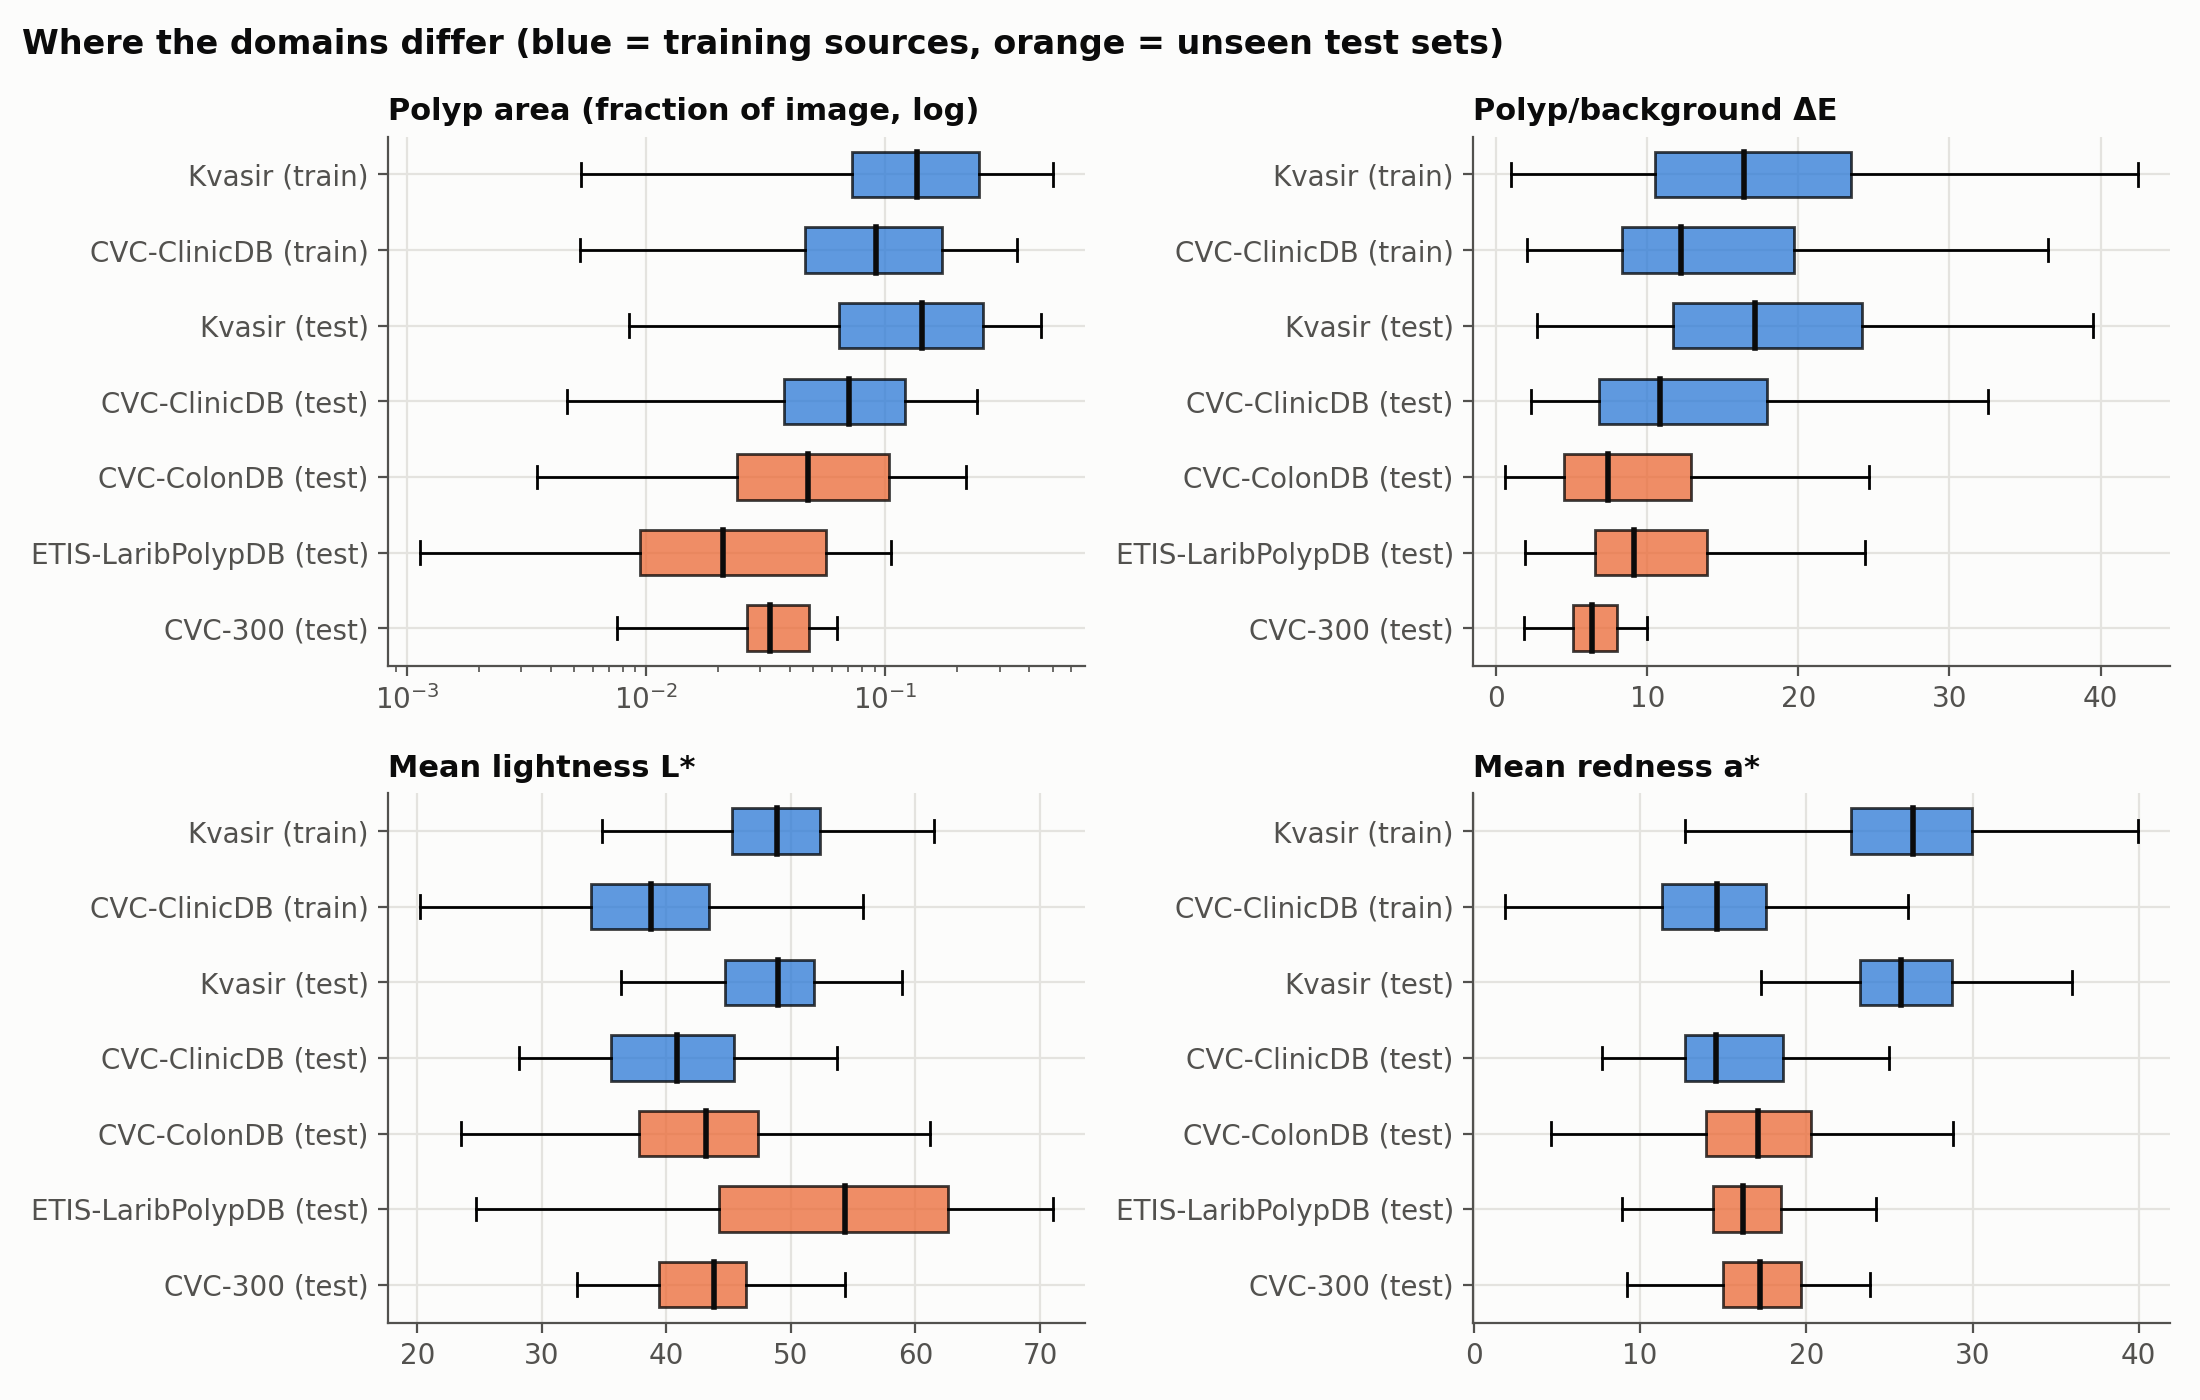
\includegraphics[width=\linewidth]{figures/dataset_stats.png}
\caption{\textbf{Domain-gap diagnosis.} Distributions of polyp size, polyp/background contrast, lightness and redness per dataset (blue: training sources, orange: unseen sets). Unseen polyps are smaller and lower in contrast.}
\label{fig:data}
\end{figure}

Before building a model we measured how the datasets differ (\cref{tab:data,fig:data}). Three differences stand out. (i) \emph{Size:} the median ColonDB polyp covers 4.7\% of the image, a third of the Kvasir median, and 21\% of ColonDB images (48\% of ETIS) contain a polyp smaller than 2\% of the image, against 2\% in Kvasir training. (ii) \emph{Contrast:} the colour difference between polyp and surrounding mucosa is about half as large in the unseen sets ($\Delta E$ 7.4 vs.\ 16.4). (iii) \emph{Colour:} Kvasir images are redder and brighter than all other sets. Resolution also differs (Kvasir $\approx$530$\times$620, ClinicDB 288$\times$384, ETIS 966$\times$1225). A model that generalizes must therefore handle small, low-contrast polyps that are rare in training.

% =====================================================================
\section{Method}
\label{sec:method}

\begin{figure*}[t]
\centering
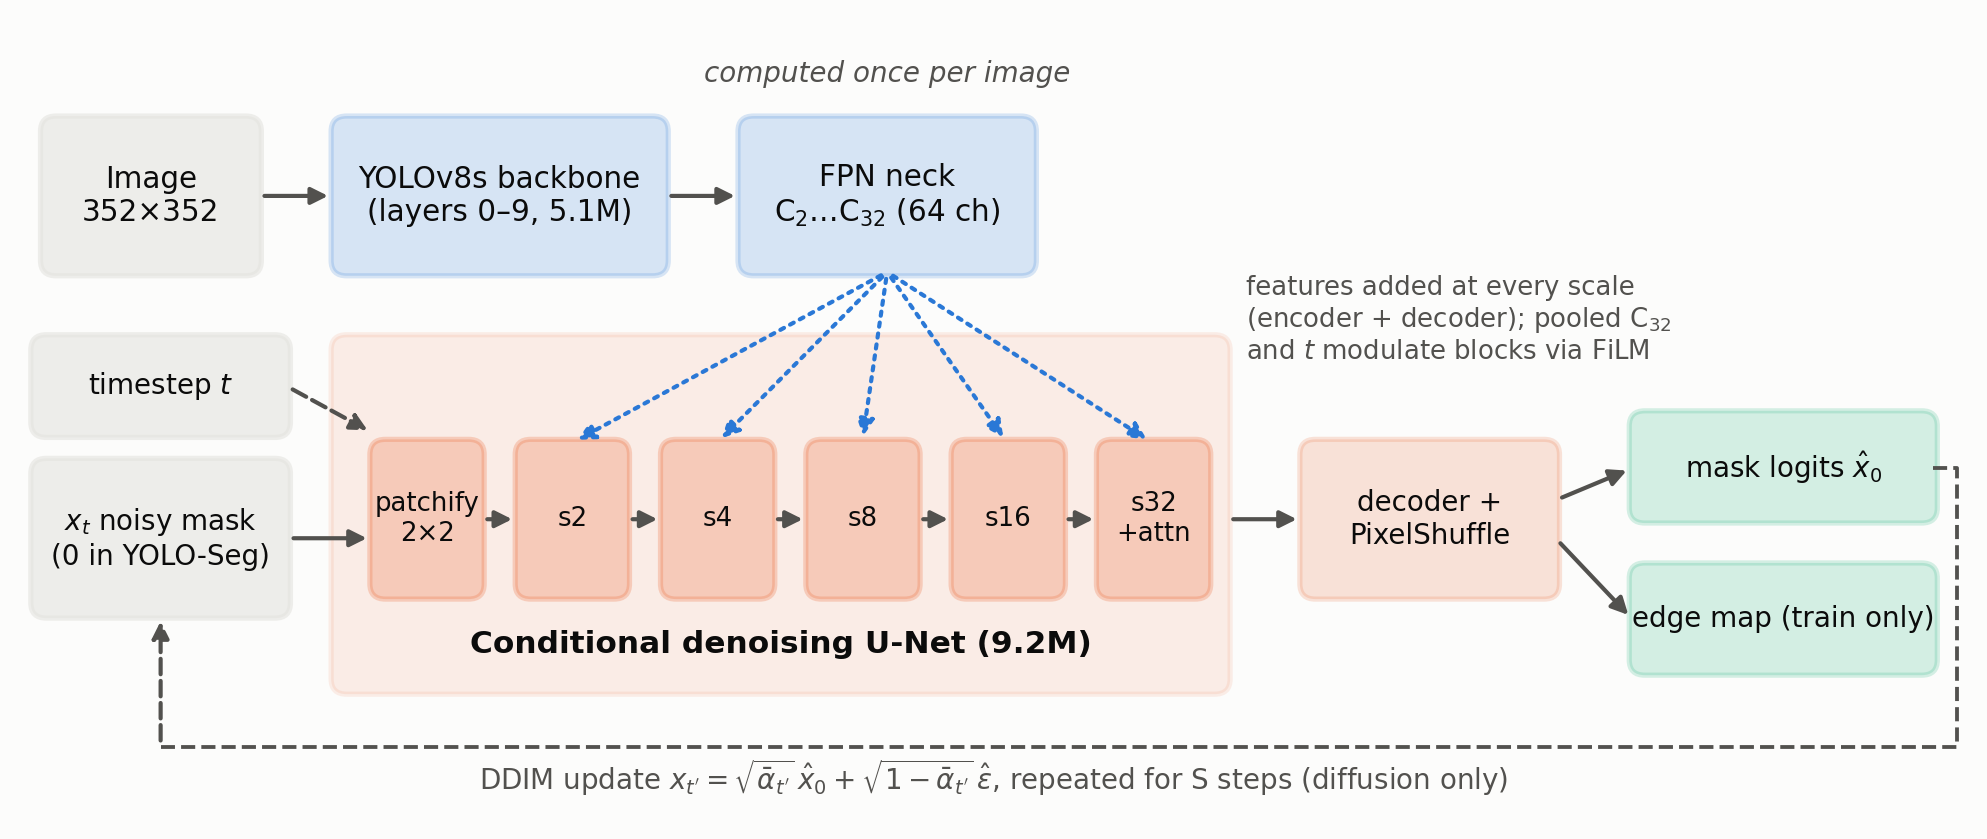
\includegraphics[width=0.9\linewidth]{figures/method.png}
\caption{\textbf{YOLO-Diff.} A YOLOv8s backbone and an FPN neck produce conditioning maps at strides 2--32 once per image. A conditional U-Net receives the noisy mask $x_t$ and the timestep $t$, adds the conditioning maps at every encoder and decoder level, and predicts the clean mask $\hat{x}_0$. In YOLO-Seg the same network receives $x_t{=}0$, $t{=}0$ and runs once.}
\label{fig:method}
\end{figure*}

\Cref{fig:method} gives an overview. Inputs are RGB images in $[0,1]$ resized to $352\times352$.

\paragraph{YOLO backbone and neck.} We take layers 0--9 of an Ultralytics YOLOv8s detector~\cite{jocher2023yolov8} pretrained on COCO, \ie the CSP backbone up to the SPPF block (5.1M parameters). Features are tapped after layers 0, 2, 4, 6 and 9 (strides 2, 4, 8, 16, 32). A top-down FPN neck~\cite{lin2017fpn} (0.25M parameters) projects each level to 64 channels, adds the upsampled coarser level, and applies a $3\times3$ convolution with GroupNorm and SiLU. This yields conditioning maps $C_2,\dots,C_{32}$ and a global vector $g$ obtained by average-pooling $C_{32}$. The backbone is fine-tuned with a 5$\times$ smaller learning rate.

\paragraph{Conditional denoiser.} The denoiser is a U-Net over the mask (9.2M parameters) with channel widths 32, 64, 128, 192, 256 at strides 2--32. A $2\times2$ patchify convolution maps the full-resolution mask to stride 2, and PixelShuffle restores the full resolution at the output. Each level has a residual block (GroupNorm, SiLU, $3\times3$ convolutions). The block is modulated by FiLM~\cite{perez2018film} scale and shift parameters computed from the sum of a sinusoidal timestep embedding and an MLP embedding of $g$. The conditioning map of the matching stride is projected by a $1\times1$ convolution and added to the block input in both the encoder and the decoder. The bottleneck at stride 32 contains multi-head self-attention. Two heads predict mask logits and, for boundary guidance, an edge map.

\paragraph{Diffusion training.} The ground-truth mask $y\in\{0,1\}$ is mapped to $x_0 = 2y-1$. We use $T=1000$ steps with the cosine schedule $\bar\alpha_t$~\cite{nichol2021improved}, and $x_t = \sqrt{\bar\alpha_t}\,x_0 + \sqrt{1-\bar\alpha_t}\,\epsilon$ with $t\sim\mathcal{U}\{0,\dots,T{-}1\}$. Instead of the noise, the network predicts the clean mask as logits $\ell = f_\theta(x_t, t, C, g)$. This lets us train with segmentation losses on $\sigma(\ell)$.

\paragraph{Sampling.} Starting from $x_{T}\sim\mathcal{N}(0,I)$ we run $S$ deterministic DDIM steps~\cite{song2021ddim} ($\eta=0$, default $S=10$). At step $t$, $\hat{x}_0 = 2\sigma(\ell)-1$, $\hat\epsilon = (x_t-\sqrt{\bar\alpha_t}\hat{x}_0)/\sqrt{1-\bar\alpha_t}$, and $x_{t'} = \sqrt{\bar\alpha_{t'}}\hat{x}_0+\sqrt{1-\bar\alpha_{t'}}\hat\epsilon$. The final prediction is $\sigma(\ell)$ at the last step. The backbone and neck run once; only the denoiser runs $S$ times. Optionally, $K$ samples with different noise are averaged.

\paragraph{Boundary guidance.} Without guidance, the loss is $\mathcal{L}_\text{BCE}+\mathcal{L}_\text{Dice}$. With guidance we use (i) the boundary-weighted structure loss of PraNet~\cite{fan2020pranet}, a weighted BCE plus weighted IoU with pixel weights $w = 1 + 5\,|\mathrm{avgpool}_{31}(y) - y|$ that emphasise pixels near the boundary, and (ii) an auxiliary edge head supervised with the 3-pixel morphological gradient of $y$ (positive-weighted BCE + Dice). The total loss is $\mathcal{L} = \mathcal{L}_\text{struct} + 0.5\,\mathcal{L}_\text{edge}$. The edge head is not used at inference.

\paragraph{YOLO-Seg ablation.} To isolate the effect of diffusion, we train the \emph{same} network with $x_t=0$ and $t=0$ for every sample. It then becomes an ordinary single-pass segmentation network with a YOLO encoder and our multi-scale decoder, with identical parameters and losses.

% =====================================================================
\section{Experimental Setup}
\label{sec:setup}

\paragraph{Baselines.} \emph{U-Net}~\cite{ronneberger2015unet}: the classic architecture (base width 64, 31.0M parameters) trained from scratch with BCE + Dice. \emph{PraNet}~\cite{fan2020pranet}: a port of the official architecture with an ImageNet-pretrained Res2Net-50 (26w$\times$4s) loaded through timm (30.5M parameters). It is trained with the structure loss on all four side outputs, as in the original code.

\paragraph{Training.} All models use the same split, resolution and augmentation: horizontal and vertical flips, shift--scale--rotate ($\pm$30$^\circ$), and brightness/contrast jitter, implemented with Albumentations~\cite{buslaev2020albumentations}. The \emph{strong} variant adds hue/saturation, gamma, blur/noise and CLAHE to simulate colour and illumination shifts. We use AdamW~\cite{loshchilov2019adamw}, batch size 16, bf16 mixed precision, gradient clipping at 1.0, and a cosine schedule with a 2-epoch warm-up. U-Net is trained for 100 epochs at learning rate $10^{-3}$, PraNet for 50 epochs at $10^{-4}$ (the official rate), and the YOLO models for 100 epochs at $5\cdot10^{-4}$ (backbone $10^{-4}$). Validation Dice is computed every 2 epochs (5 DDIM steps for diffusion models), and the best checkpoint is kept. Every configuration is trained with seeds 0, 1 and 2. Training used PyTorch~\cite{paszke2019pytorch} on one NVIDIA RTX 5000 Ada GPU shared with other users.

\paragraph{Metrics.} Predictions are upsampled to the original mask size and thresholded at 0.5. All metrics are computed per image and averaged. We report Dice, IoU, the Boundary F-score~\cite{csurka2013bf} (BF; tolerance 0.75\% of the image diagonal), and HD95, the symmetric 95th-percentile boundary distance in pixels. A missed polyp receives the image diagonal as its HD95. ``Seen'' pools the 162 Kvasir and ClinicDB test images. Latency is the mean fp32 forward time for one $352\times352$ image (batch 1, 50 runs after 10 warm-up runs). Diffusion models are evaluated with a fixed noise seed.

% =====================================================================
\section{Results}
\label{sec:results}

\begin{table*}[t]
\centering
\footnotesize
\setlength{\tabcolsep}{4pt}
\begin{tabular}{@{}lrr|cc|cccc|cc|c@{}}
\toprule
& & & \multicolumn{2}{c|}{Seen (162)} & \multicolumn{4}{c|}{\textbf{CVC-ColonDB} (380, unseen)} & \multicolumn{2}{c|}{ETIS (196)} & CVC-300 \\
Method & Params & Latency & Dice & BF & Dice & IoU & BF & HD95$\downarrow$ & Dice & HD95$\downarrow$ & Dice \\
\midrule
U-Net~\cite{ronneberger2015unet} & 31.0M & 5 ms & .844\pmstd{.002} & .673 & .649\pmstd{.016} & .562 & .515 & 157.6 & .492\pmstd{.022} & 467.0 & .813 \\
PraNet~\cite{fan2020pranet} & 30.5M & 19 ms & .903\pmstd{.005} & .815 & .747\pmstd{.009} & .676 & .630 & 109.3 & \best{.703}\pmstd{.020} & 284.1 & \best{.884} \\
\midrule
YOLO-Seg (no diffusion) & 14.5M & 19 ms & \best{.910}\pmstd{.001} & \best{.832} & \best{.777}\pmstd{.004} & \best{.699} & \best{.656} & \best{74.2} & .697\pmstd{.022} & 224.2 & .880 \\
YOLO-Diff, no boundary & 14.5M & 140 ms & .849\pmstd{.006} & .725 & .714\pmstd{.014} & .630 & .591 & 103.5 & .666\pmstd{.007} & 229.5 & .859 \\
YOLO-Diff, boundary & 14.5M & 140 ms & .861\pmstd{.007} & .761 & .740\pmstd{.007} & .655 & .624 & 87.6 & .683\pmstd{.007} & 224.5 & .860 \\
YOLO-Diff, boundary + strong aug. & 14.5M & 140 ms & .862\pmstd{.001} & .752 & .754\pmstd{.008} & .666 & .621 & 76.5 & .700\pmstd{.020} & \best{213.0} & .855 \\
\bottomrule
\end{tabular}
\caption{\textbf{Main results}, mean over 3 seeds ($\pm$ std for Dice). All models were trained on Kvasir + ClinicDB only. HD95 is in pixels at the original resolution. Latency: batch 1, fp32, 10 DDIM steps for YOLO-Diff, measured on a shared GPU (relative values are meaningful, absolute values are noisy).}
\label{tab:main}
\end{table*}

\Cref{tab:main} gives the main results. Our PraNet re-implementation reaches 0.747 Dice on ColonDB and 0.703 on ETIS, close to or above the values reported in the original paper (0.709 and 0.628). This confirms that the baseline is well tuned and that our evaluation is comparable.

\paragraph{The YOLO backbone generalizes better at half the size.} YOLO-Seg improves over PraNet on the unseen ColonDB in every metric: Dice +0.030, IoU +0.023, BF +0.026, and HD95 lower by 32\% (74.2 vs.\ 109.3 px). It is also slightly better on the seen data. It does so with 14.5M instead of 30.5M parameters, and its backbone is 4.7$\times$ smaller than Res2Net-50 (5.1M vs.\ 23.7M), at the same latency. On ETIS and CVC-300 the Dice of YOLO-Seg and PraNet are within one standard deviation, while YOLO-Seg again has a lower HD95 (224 vs.\ 284 on ETIS). U-Net trained from scratch generalizes worst, especially on ETIS (0.492), where small polyps dominate.

\begin{table}[t]
\centering
\footnotesize
\setlength{\tabcolsep}{3.5pt}
\begin{tabular}{@{}lccc@{}}
\toprule
Method & Seen & ColonDB & Gap $\downarrow$ \\
\midrule
U-Net & .844 & .649 & .195\pmstd{.016} \\
PraNet & .903 & .747 & .156\pmstd{.012} \\
YOLO-Seg & .910 & .777 & .133\pmstd{.004} \\
YOLO-Diff, no boundary & .849 & .714 & .136\pmstd{.014} \\
YOLO-Diff, boundary & .861 & .740 & .121\pmstd{.005} \\
YOLO-Diff, bnd.\ + strong aug. & .862 & .754 & \best{.108}\pmstd{.008} \\
\bottomrule
\end{tabular}
\caption{\textbf{Generalization gap} (seen Dice $-$ ColonDB Dice, computed per seed). A small gap is only desirable when seen accuracy is also high; see text.}
\label{tab:gap}
\end{table}

\paragraph{Diffusion does not help.} Holding everything else fixed, turning YOLO-Seg into a diffusion model lowers ColonDB Dice from 0.777 to 0.740 and seen Dice from 0.910 to 0.861, while latency grows 7$\times$. \Cref{tab:sweep} varies the number of DDIM steps. A single step, \ie predicting the mask from pure noise in one pass, is as accurate as 10 or 20 steps, and more steps even reduce BF slightly. Averaging 5 samples gains only +0.005 Dice. The model has therefore learnt to rely on the image features and to largely ignore the noisy mask input. The iterative refinement that motivated the diffusion formulation does not materialise. We see two likely reasons. First, the conditioning features already determine the mask almost uniquely, since a polyp mask is a simple, mostly convex region, so there is little multi-modality for sampling to resolve. Second, training a denoiser over all noise levels spreads the 100-epoch budget over a harder task than single-pass segmentation.

\begin{table}[t]
\centering
\footnotesize
\setlength{\tabcolsep}{4pt}
\begin{tabular}{@{}lcccr@{}}
\toprule
Sampling & ColonDB Dice & ColonDB BF & Seen Dice & ms \\
\midrule
1 step & .743\pmstd{.007} & .625 & .865 & 18 \\
3 steps & .742\pmstd{.006} & .625 & .863 & 45 \\
5 steps & .741\pmstd{.006} & .630 & .862 & 72 \\
10 steps (default) & .740\pmstd{.007} & .624 & .861 & 140 \\
20 steps & .736\pmstd{.007} & .614 & .859 & 255 \\
10 steps $\times$ 5 samples & .745\pmstd{.006} & .639 & .866 & 138 \\
\bottomrule
\end{tabular}
\caption{\textbf{DDIM steps and ensembling} for YOLO-Diff (boundary), 3 seeds. The 5 samples are run as one batch, so their latency is close to a single sample on our GPU.}
\label{tab:sweep}
\end{table}

\paragraph{Boundary guidance and appearance augmentation help.} Within the diffusion model, boundary guidance raises ColonDB Dice by 0.026, BF by 0.033, and lowers HD95 from 103.5 to 87.6 px. The improvement is consistent on the seen data, ETIS and CVC-300. Strong appearance augmentation adds a further +0.014 Dice on ColonDB and +0.017 on ETIS, and lowers HD95 to 76.5, without changing seen accuracy. This is the expected effect of simulating colour and illumination shift. \Cref{tab:gap} shows that this model also has the smallest seen--unseen gap (0.108). Part of this small gap, however, comes from its lower seen accuracy. YOLO-Seg remains the best model in absolute terms on both seen and unseen data. Combining YOLO-Seg with strong augmentation is a natural next experiment that we did not run.

\begin{figure}[t]
\centering
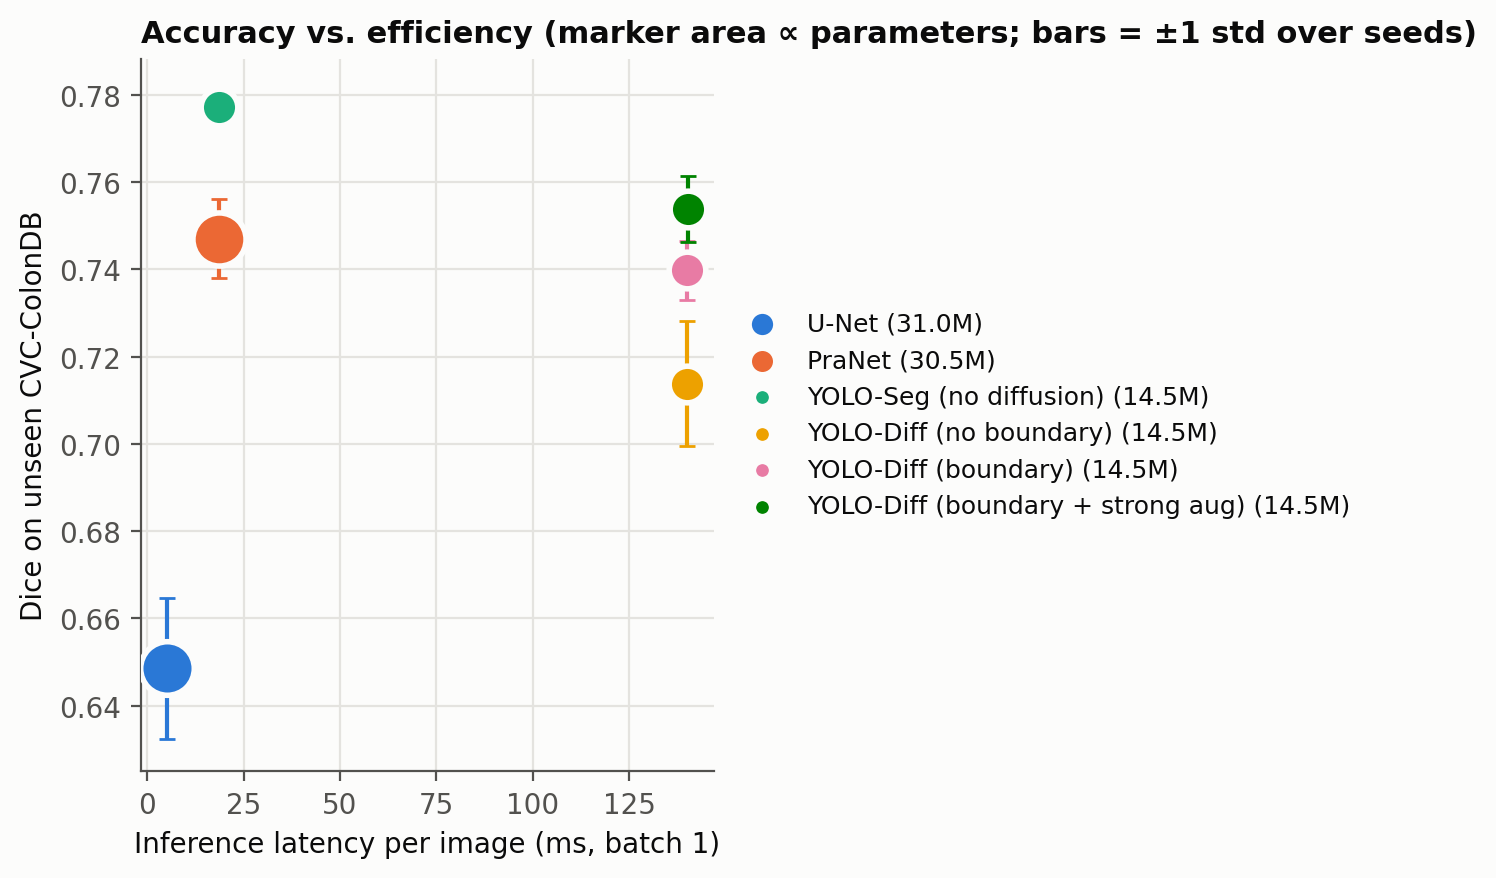
\includegraphics[width=\linewidth]{figures/accuracy_efficiency.png}
\caption{\textbf{Accuracy vs.\ efficiency} on ColonDB. Marker area is proportional to the number of parameters; error bars show $\pm$1 std over seeds.}
\label{fig:eff}
\end{figure}

\paragraph{Accuracy vs.\ efficiency.} \Cref{fig:eff} summarises the trade-off. YOLO-Seg is the only model that is both more accurate than PraNet and smaller. The diffusion variants are smaller than PraNet but 7$\times$ slower with 10 steps. Since one step is as accurate as ten (\cref{tab:sweep}), YOLO-Diff can run at YOLO-Seg's latency (18 ms) without losing accuracy, although YOLO-Seg remains more accurate.

% =====================================================================
\section{Error Analysis}
\label{sec:errors}

\begin{table}[t]
\centering
\footnotesize
\setlength{\tabcolsep}{3pt}
\begin{tabular}{@{}lccc|ccc@{}}
\toprule
& \multicolumn{3}{c|}{Polyp area} & \multicolumn{3}{c}{Contrast $\Delta E$ tertile} \\
Method & $<$2\% & 2--8\% & $>$8\% & low & mid & high \\
& (79) & (182) & (119) & (127) & (126) & (126) \\
\midrule
U-Net & .471 & .786 & .556 & .655 & .726 & .570 \\
PraNet & .555 & \best{.861} & .700 & .737 & .801 & .709 \\
YOLO-Seg & \best{.635} & .857 & \best{.750} & \best{.784} & \best{.802} & \best{.751} \\
YOLO-Diff, no bnd. & .541 & .846 & .626 & .703 & .758 & .687 \\
YOLO-Diff, bnd. & .565 & .844 & .697 & .733 & .766 & .727 \\
YOLO-Diff, + aug. & .594 & .851 & .711 & .746 & .772 & .750 \\
\bottomrule
\end{tabular}
\caption{\textbf{ColonDB Dice by polyp size and by polyp/background contrast} (seed-averaged per image; number of images in parentheses; one image has no valid contrast ring).}
\label{tab:buckets}
\end{table}

\paragraph{Small polyps explain most of the gap.} \Cref{tab:buckets} splits ColonDB by polyp size and contrast. All methods are accurate on medium polyps (0.84--0.86 for all but U-Net), and the differences between methods arise almost entirely on small and large polyps. On small polyps, the regime that is 10$\times$ more frequent in ColonDB than in Kvasir training, YOLO-Seg reaches 0.635 against 0.555 for PraNet. We attribute this to the detector backbone: YOLO is pretrained to localise objects at many scales and keeps a high-resolution stride-2 feature map, which our decoder uses directly. For YOLO-Diff (boundary), 18.4\% of ColonDB images are failures (Dice $<$0.5). Their median polyp area is 2.3\%, against 4.8\% for successful cases. YOLO-Seg is also the most robust to low contrast (0.784 vs.\ 0.737 for PraNet in the lowest tertile).

\paragraph{Large polyps also fail.} Surprisingly, large polyps ($>$8\%) score lower than medium ones for every method. Eight of the 15 worst ColonDB images for YOLO-Diff are consecutive frames 301--320, in which the polyp covers 20--60\% of the image (\cref{fig:qual}, rows 5--6). These are flat, low-texture lesions that fill the field of view, a configuration that is rare in training, where polyps are usually seen as compact protrusions. Every method misses them almost completely.

\begin{figure*}[t]
\centering
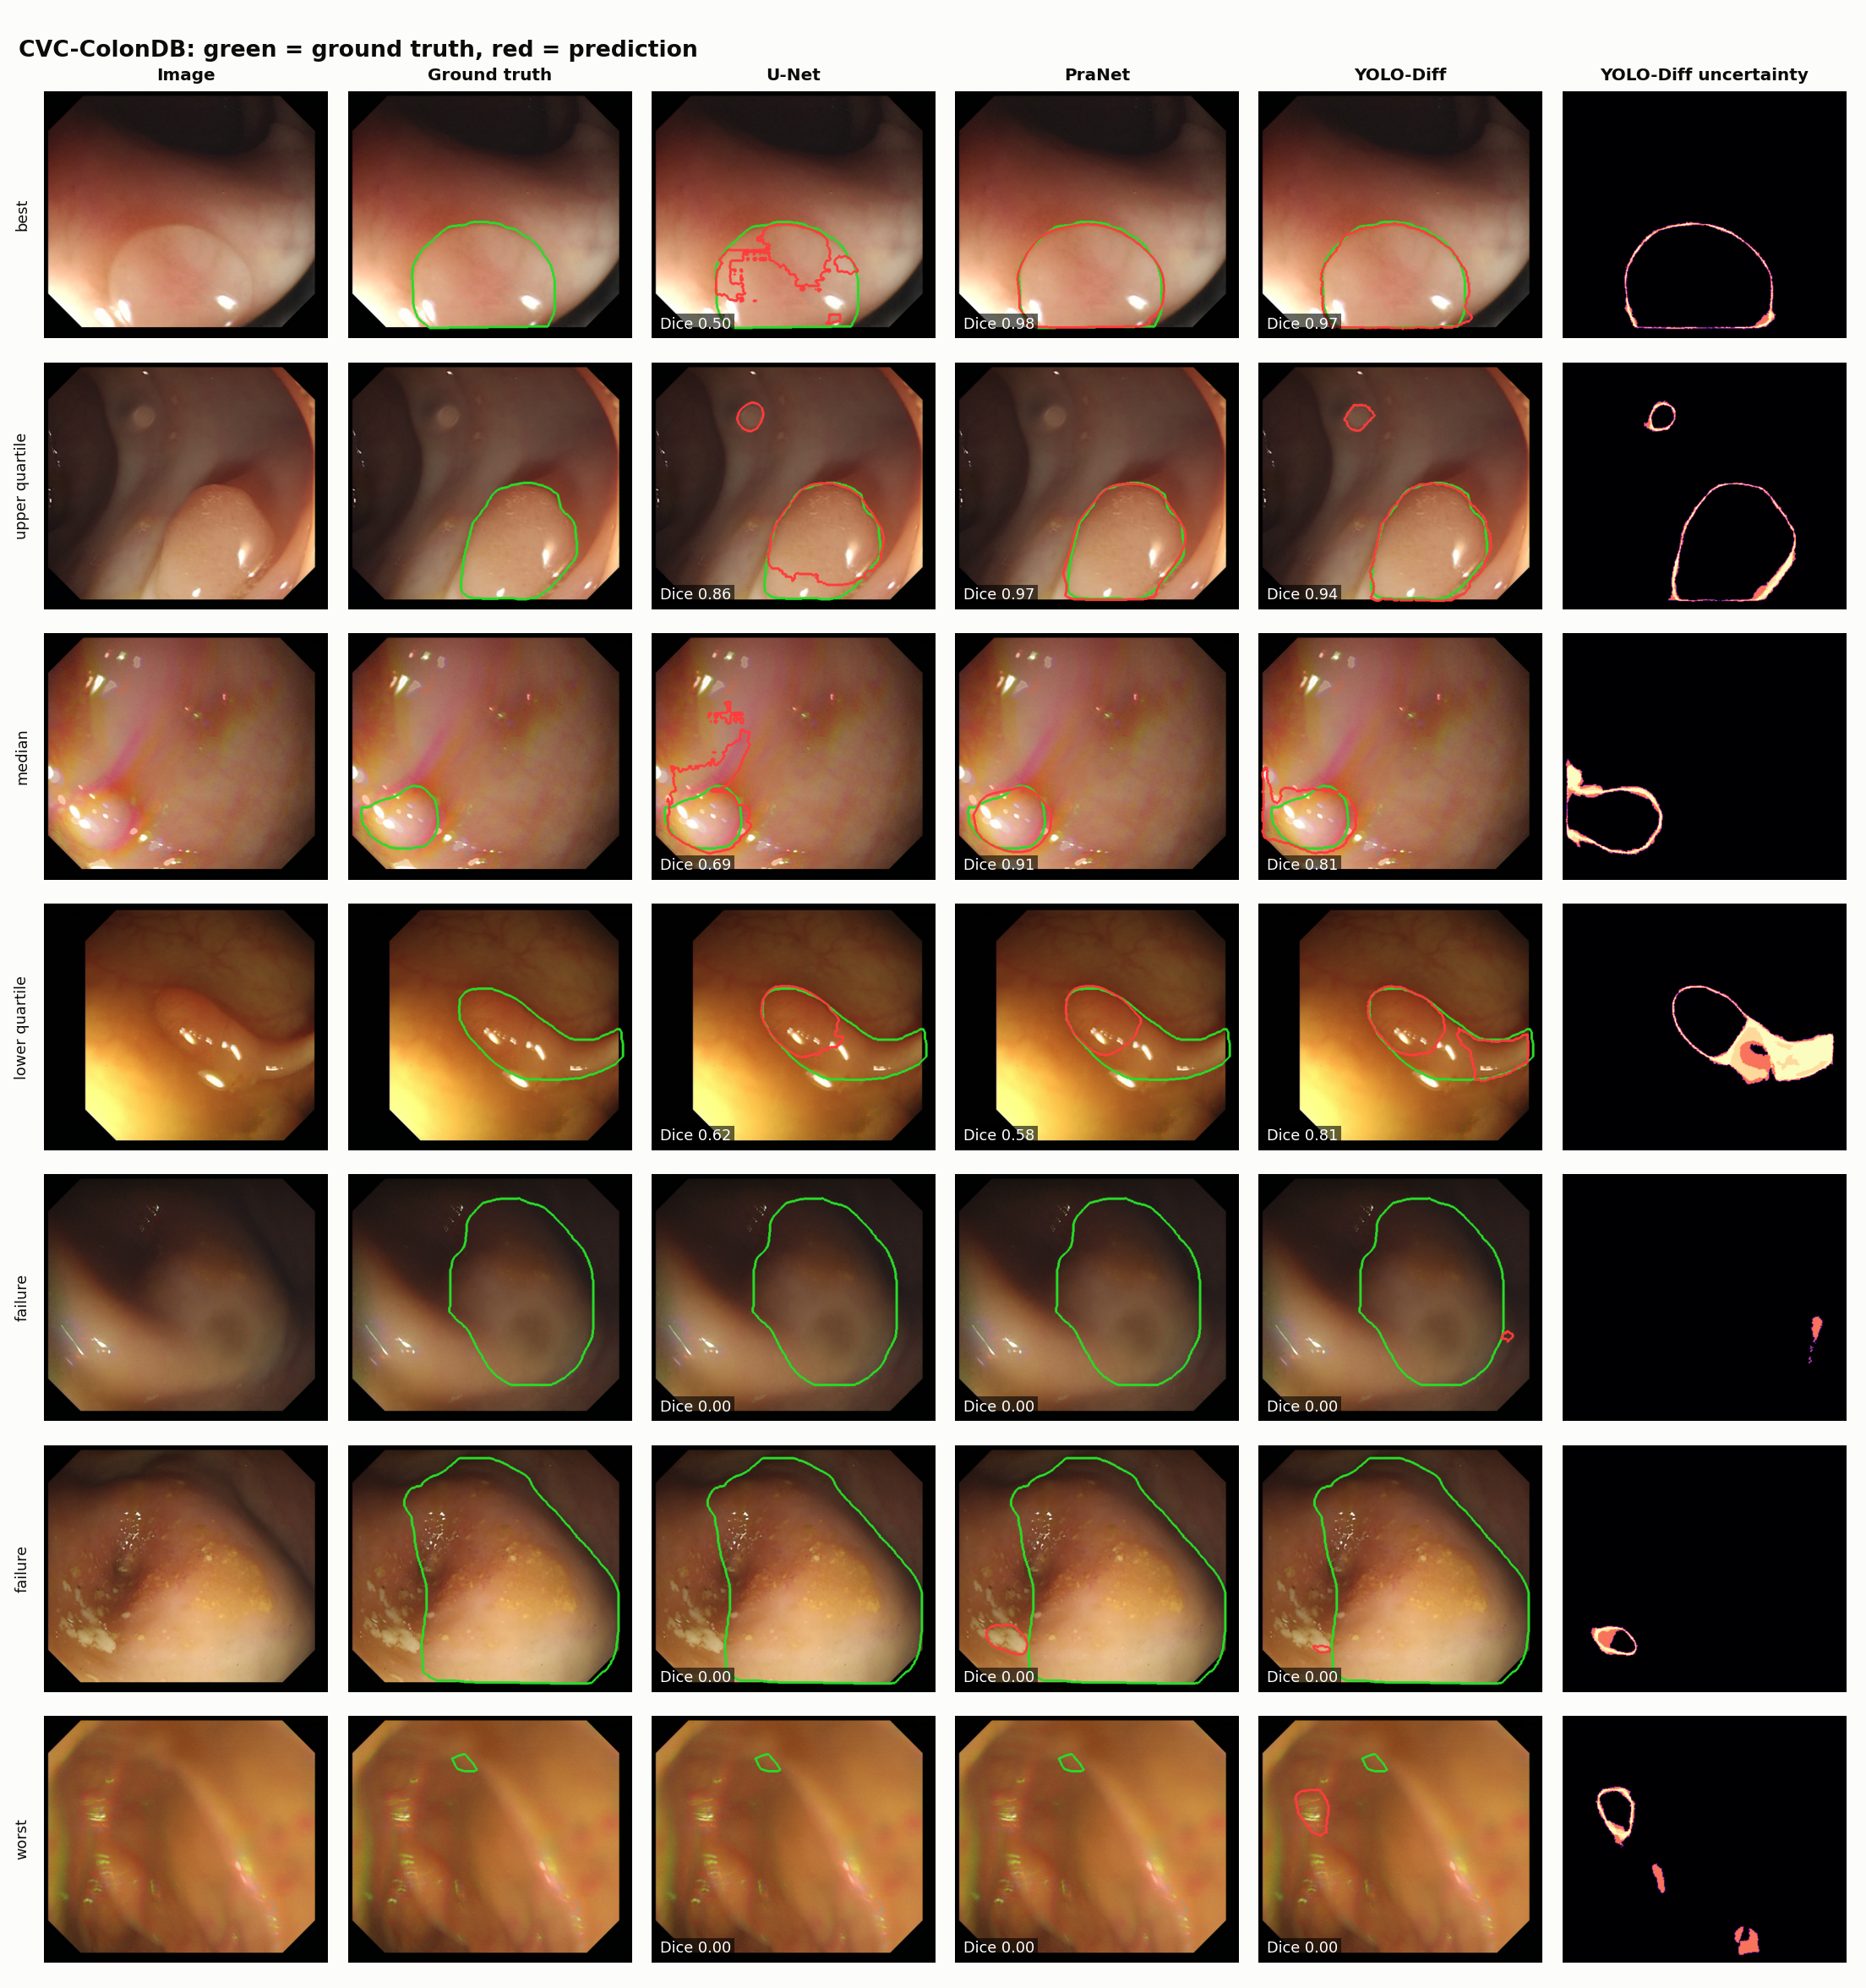
\includegraphics[width=0.82\linewidth]{figures/qualitative_colondb.png}
\caption{\textbf{Qualitative results on CVC-ColonDB} (seed-0 models), from the best to the worst image of YOLO-Diff (boundary). Green: ground truth; red: prediction. The last column shows the pixel-wise standard deviation over 8 diffusion samples. Uncertainty concentrates on the predicted boundary and on false-positive regions (rows 3, 4, 7), but it is near zero where a large polyp is missed entirely (rows 5, 6).}
\label{fig:qual}
\end{figure*}

\paragraph{Diffusion uncertainty.} One expected benefit of diffusion is a per-pixel uncertainty estimate from multiple samples. \Cref{fig:qual} shows that the sample variance highlights boundaries and some false positives. However, it is almost zero on the large missed polyps, so the model is confidently wrong there. This limits its usefulness as a failure detector.

% =====================================================================
\section{Discussion and Limitations}
\label{sec:discussion}

Our proposal had two parts, a lightweight YOLO backbone and diffusion-based mask generation. The experiments support the first and not the second. Measured against the success criterion of our project plan (improved boundary quality and maintained or improved Dice on unseen ColonDB without substantial extra computation), YOLO-Seg meets all three conditions. YOLO-Diff maintains Dice (0.740 vs.\ 0.747, within one standard deviation of PraNet) and improves HD95, but does not improve BF and costs 7$\times$ more computation with 10 steps.

\paragraph{Limitations.} (i) We evaluate cross-\emph{dataset}, not cross-\emph{centre}: the PraNet test sets do not identify acquisition sites, and ColonDB consists of frames from a limited number of video sequences, so the images are not independent. (ii) PraNet is trained with our shared protocol, without its multi-scale training, and all models use a fixed 0.5 threshold. (iii) The diffusion hyperparameters (noise schedule, signal scaling, $x_0$ parameterisation, number of epochs) were not tuned, and other choices such as self-conditioning or signal scaling might make the iterative process useful. (iv) Latency was measured on a GPU shared with other jobs. (v) We did not evaluate on PolypGen~\cite{ali2023polypgen} or compare with stronger transformer-based models.

% =====================================================================
\section{Conclusion}
\label{sec:conclusion}

We studied cross-dataset polyp segmentation with a YOLO-backbone-guided conditional diffusion model under a strict protocol with three seeds. The domain-gap analysis showed that the unseen datasets contain far more small and low-contrast polyps. A YOLOv8s backbone with a multi-scale decoder addresses this better than PraNet's Res2Net-50 (ColonDB Dice 0.777 vs.\ 0.747, HD95 74 vs.\ 109) with half the parameters. Iterative diffusion sampling, in contrast, did not improve accuracy in our setting: one step matches twenty. Boundary guidance and appearance augmentation were the most effective additions. Future work should combine the YOLO backbone with appearance augmentation, target large flat polyps, and test on multi-centre data.

% =====================================================================
\section{Reproducibility Statement}
\label{sec:repro}

\paragraph{Artifacts.} Code, configuration, logs and per-image results: \repoURL. Trained checkpoints (18 $\times$ 56--119\,MB, 1.4\,GB in total, above GitHub's 100\,MB file limit): \hfURL, with SHA-256 digests in \texttt{checkpoints.sha256}. The environment is pinned in \texttt{requirements.txt} and \texttt{environment.yml} (Python 3.9.22, PyTorch 2.6.0, CUDA 12.4, timm 0.6.12, ultralytics 8.4.24). The datasets are not redistributed; \texttt{scripts/download\_data.sh} fetches the public PraNet split, and checksums are provided.

\paragraph{Instructions.} \texttt{bash scripts/download\_data.sh} downloads the data and YOLOv8 weights. \texttt{bash scripts/reproduce\_eval.sh HF\_REPO\_ID} regenerates every table and figure from the released checkpoints in about 30 minutes. \texttt{bash run\_all.sh} retrains all 18 models (about 6 hours on our shared GPU) and then evaluates them.

\paragraph{Verification.} Re-evaluating saved checkpoints gave bit-identical per-image metrics, including for the diffusion model, which uses a fixed noise seed. Re-training is not bit-exact because of non-deterministic cuDNN kernels; we therefore report the standard deviation over three seeds.

\paragraph{Declaration.} We declare that all results in this report were produced by the code in the repository at the commits listed in \cref{tab:commits}, that no test data was used for training, hyperparameter choice or checkpoint selection, that all runs are reported, and that the released checkpoints are the ones evaluated here.

\begin{table}[h]
\centering
\scriptsize
\setlength{\tabcolsep}{2pt}
\begin{tabular}{@{}l l p{0.55\linewidth}@{}}
\toprule
Hash & Timestamp & Message \\
\midrule
\texttt{01170b3} & 2026-11-21 10:17:05 +0530 & Project setup: environment files, data download script, checksums \\
\texttt{ccf89bc} & 2026-11-21 10:17:05 +0530 & Data pipeline: PraNet split loading, fixed train/val split, augmentation \\
\texttt{85c8b8d} & 2026-11-21 10:17:05 +0530 & Metrics (Dice, IoU, Boundary F, HD95) and losses (BCE+Dice, structure, edge) \\
\texttt{c90ef2c} & 2026-11-21 10:17:05 +0530 & Baselines: U-Net and PraNet (port of official architecture) \\
\texttt{82fbc04} & 2026-11-21 10:17:05 +0530 & Proposed model: YOLOv8-backbone-guided conditional diffusion with DDIM sampling \\
\texttt{0274caa} & 2026-11-21 10:17:05 +0530 & Training and evaluation scripts, full experiment pipeline \\
\texttt{0a52dbc} & 2026-11-21 10:17:05 +0530 & Analysis: result tables, domain-gap statistics, error analysis, figures \\
\texttt{6bad146} & 2026-11-21 10:17:06 +0530 & Experiment artifacts: per-run configs, training curves, per-image test metrics, logs \\
\texttt{f12a87e} & 2026-11-21 10:17:06 +0530 & Results: final tables and figures (18 runs, 3 seeds) \\
\texttt{5de083d} & 2026-11-21 10:17:06 +0530 & Reproducibility: checkpoint hosting, eval-only reproduction, commit table script \\
\texttt{d7b66e8} & 2026-11-21 10:17:06 +0530 & Documentation: README with reproduction instructions, reproducibility declaration \\
\texttt{e68a642} & 2026-11-21 10:24:03 +0530 & Report: CVPR-format paper (LaTeX), method figure, bibliography, commit table \\
\texttt{05ef955} & 2026-11-21 10:24:03 +0530 & Report: update commit table \\
\texttt{6bac315} & 2026-11-26 19:53:21 +0530 & Report: add GitHub repository link \\
\texttt{ba753a6} & 2026-11-26 19:53:21 +0530 & Report: update commit table \\
\texttt{3a2ff83} & 2026-11-26 20:14:06 +0530 & Add Hugging Face checkpoint link to README and report \\
\bottomrule
\end{tabular}

\caption{\textbf{Commit history} (hash, timestamp in IST, message) at the time of writing. The commits that add this report and its final commit table follow these.}
\label{tab:commits}
\end{table}

{
    \small
    \bibliographystyle{ieeenat_fullname}
    \bibliography{refs}
}

\end{document}
